\section{Studies} % (fold)
\label{sec:studies}

To begin understanding what a deep network can learn about jet topology, we choose a finite region of phase space, and standardize our comparisons. In an effort to define a standard way that physics object identification using machine learning should be conducted, we exactly define our procedure for comparisons. In particular, we restrict our studies to $250$ GeV $\leq p_T \leq 300$ GeV, and confine ourselves to a $65$ GeV $\leq m \leq 95$ GeV mass window, wholly containing the peak of the $W$. 

We construct a scaffolded and multi-approach series of methodologies for understanding, visualizing, and validating neural networks within HEP.

\subsection{Coarse Studies} % (fold)
\label{sub:coarse_studies}

To a first order, the first desirable characteristic is a simple performance improvement over the standard physics-driven variables for discrimination. In particular, we compare our network to $n$-subjettiness~\cite{nsub} and the jet mass. We henceforth refer to $n$-subjettiness as $\tau_{21}$ for our purposes, as $\tau_{2}/\tau_{1}$ is relevant for our classification problem.

In Figure~\ref{fig:combinedROC}, we illustrate the performance gains of a deep neural network over both $\tau_{21}$ and the 2D likelihood of $\tau_{21}$ and jet mass. 


\begin{figure}[!htbp]
  \centering
  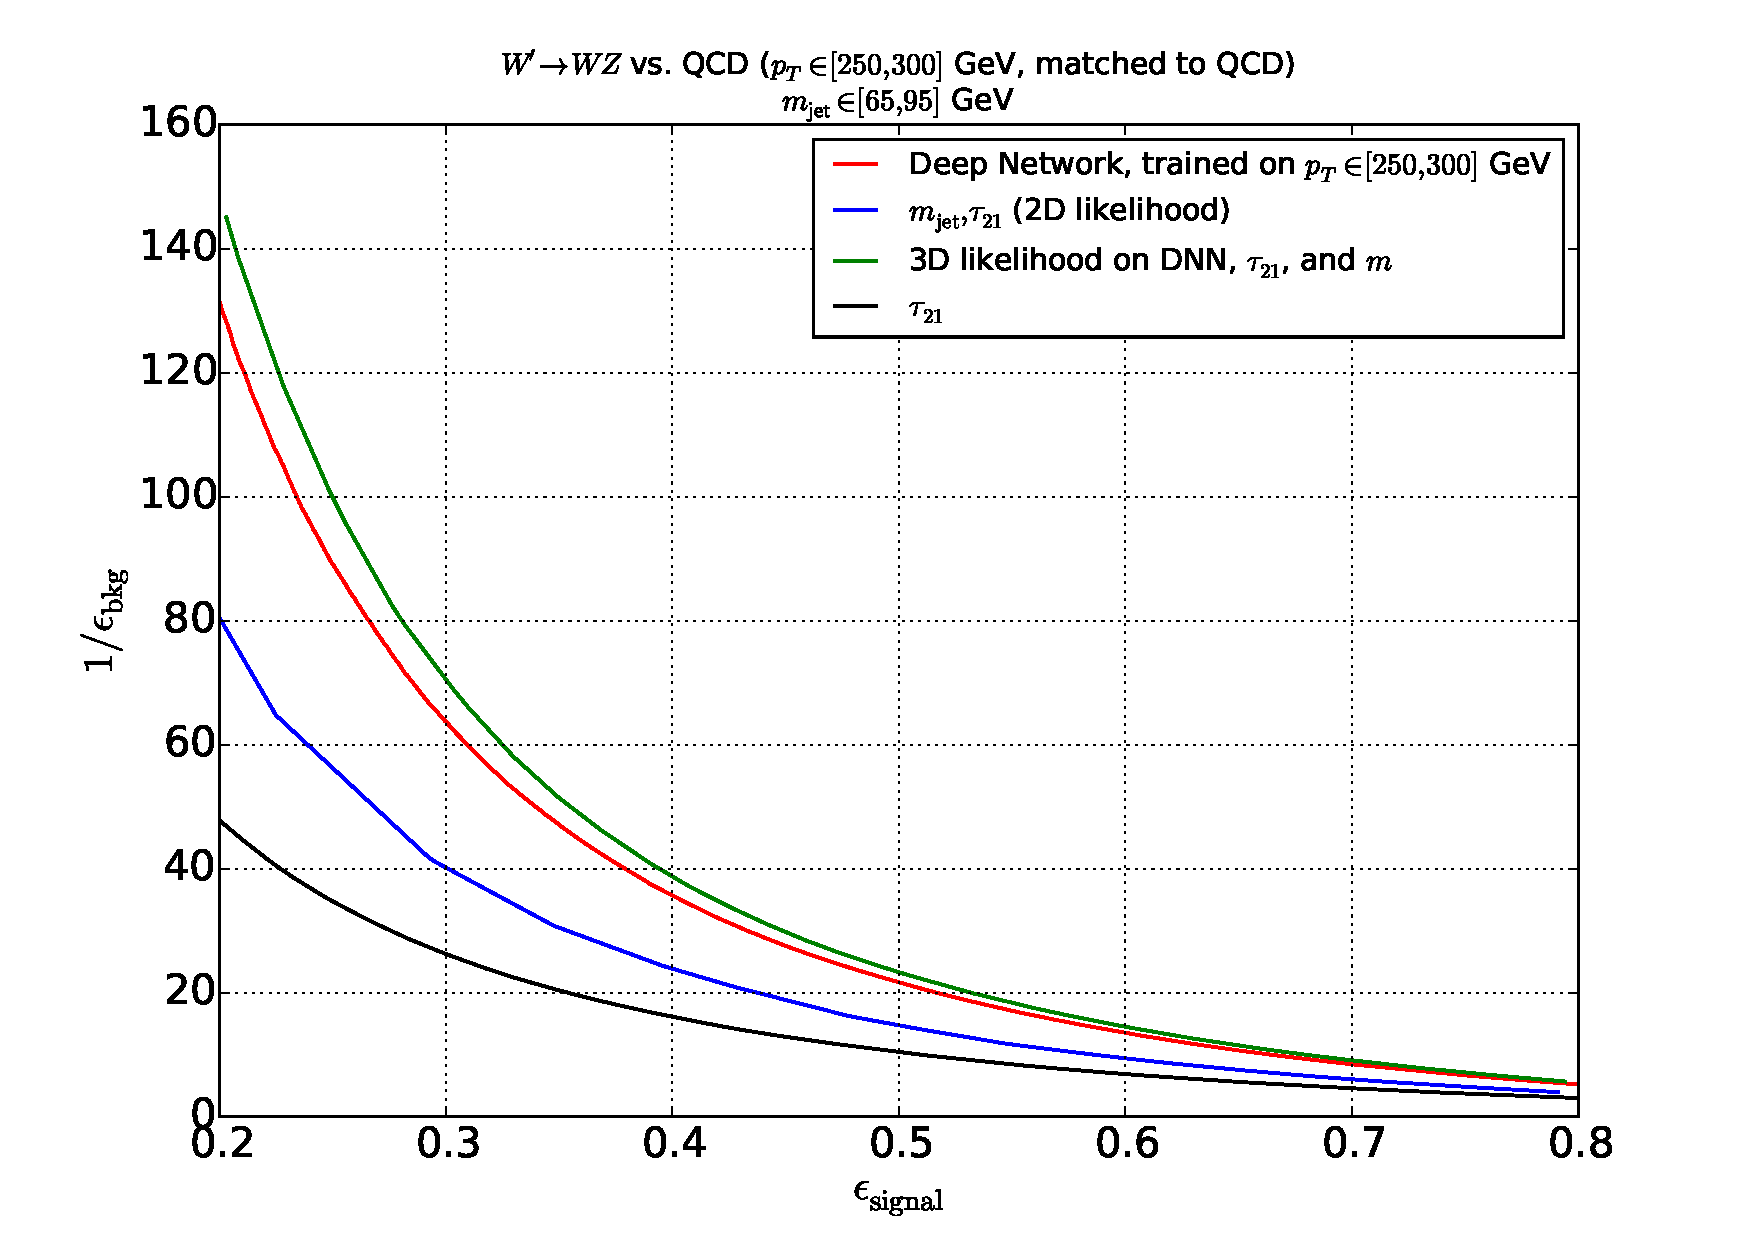
\includegraphics[width=0.95\textwidth]{figures/combined-roc.pdf}
  \caption{Receiver Operating Characteristic (ROC) over coarse sample}
  \label{fig:combinedROC}
\end{figure}

We also provide a comparison to a 3D likelihood constructed on $\tau_{21}$, jet mass, and the deep network output itself. We can gain a significant piece of insight from this. Note how in Figure~\ref{fig:combinedROC} we can see that the DNN represents a large gain on a physics-only likelihood. However, when we explicitly include the physics variable in a 3D likelihood, we see a small but definitively non-zero performance gain. This implies that the performance boost \emph{by definition} is getting its gain from something that is not \emph{fully} encapsulated in $\tau_{21}$ and jet mass. 

Though important on it's own, this figure of merit does little to help drive understanding in the context of HEP. Such an increase begs further questions -- what is this gain, and where does it come from? Why is the DNN able to pick up on this?



\subsubsection{Understanding what is learned} % (fold)
\label{ssub:understanding_what_is_learned}

% subsubsection understanding_what_is_learned (end)
In Figure~\ref{fig:convkernels}, we first examine the $11\times11$ convolutional filters in the first layer and look for structure. In

In order to understand what we learn, we first take a look \emph{inside} the deep network. 
\begin{figure}[bt]
  \begin{center}
      \subfloat[$(11\times11)$ convolutional kernels from first layer \label{subfig:filters}]{
        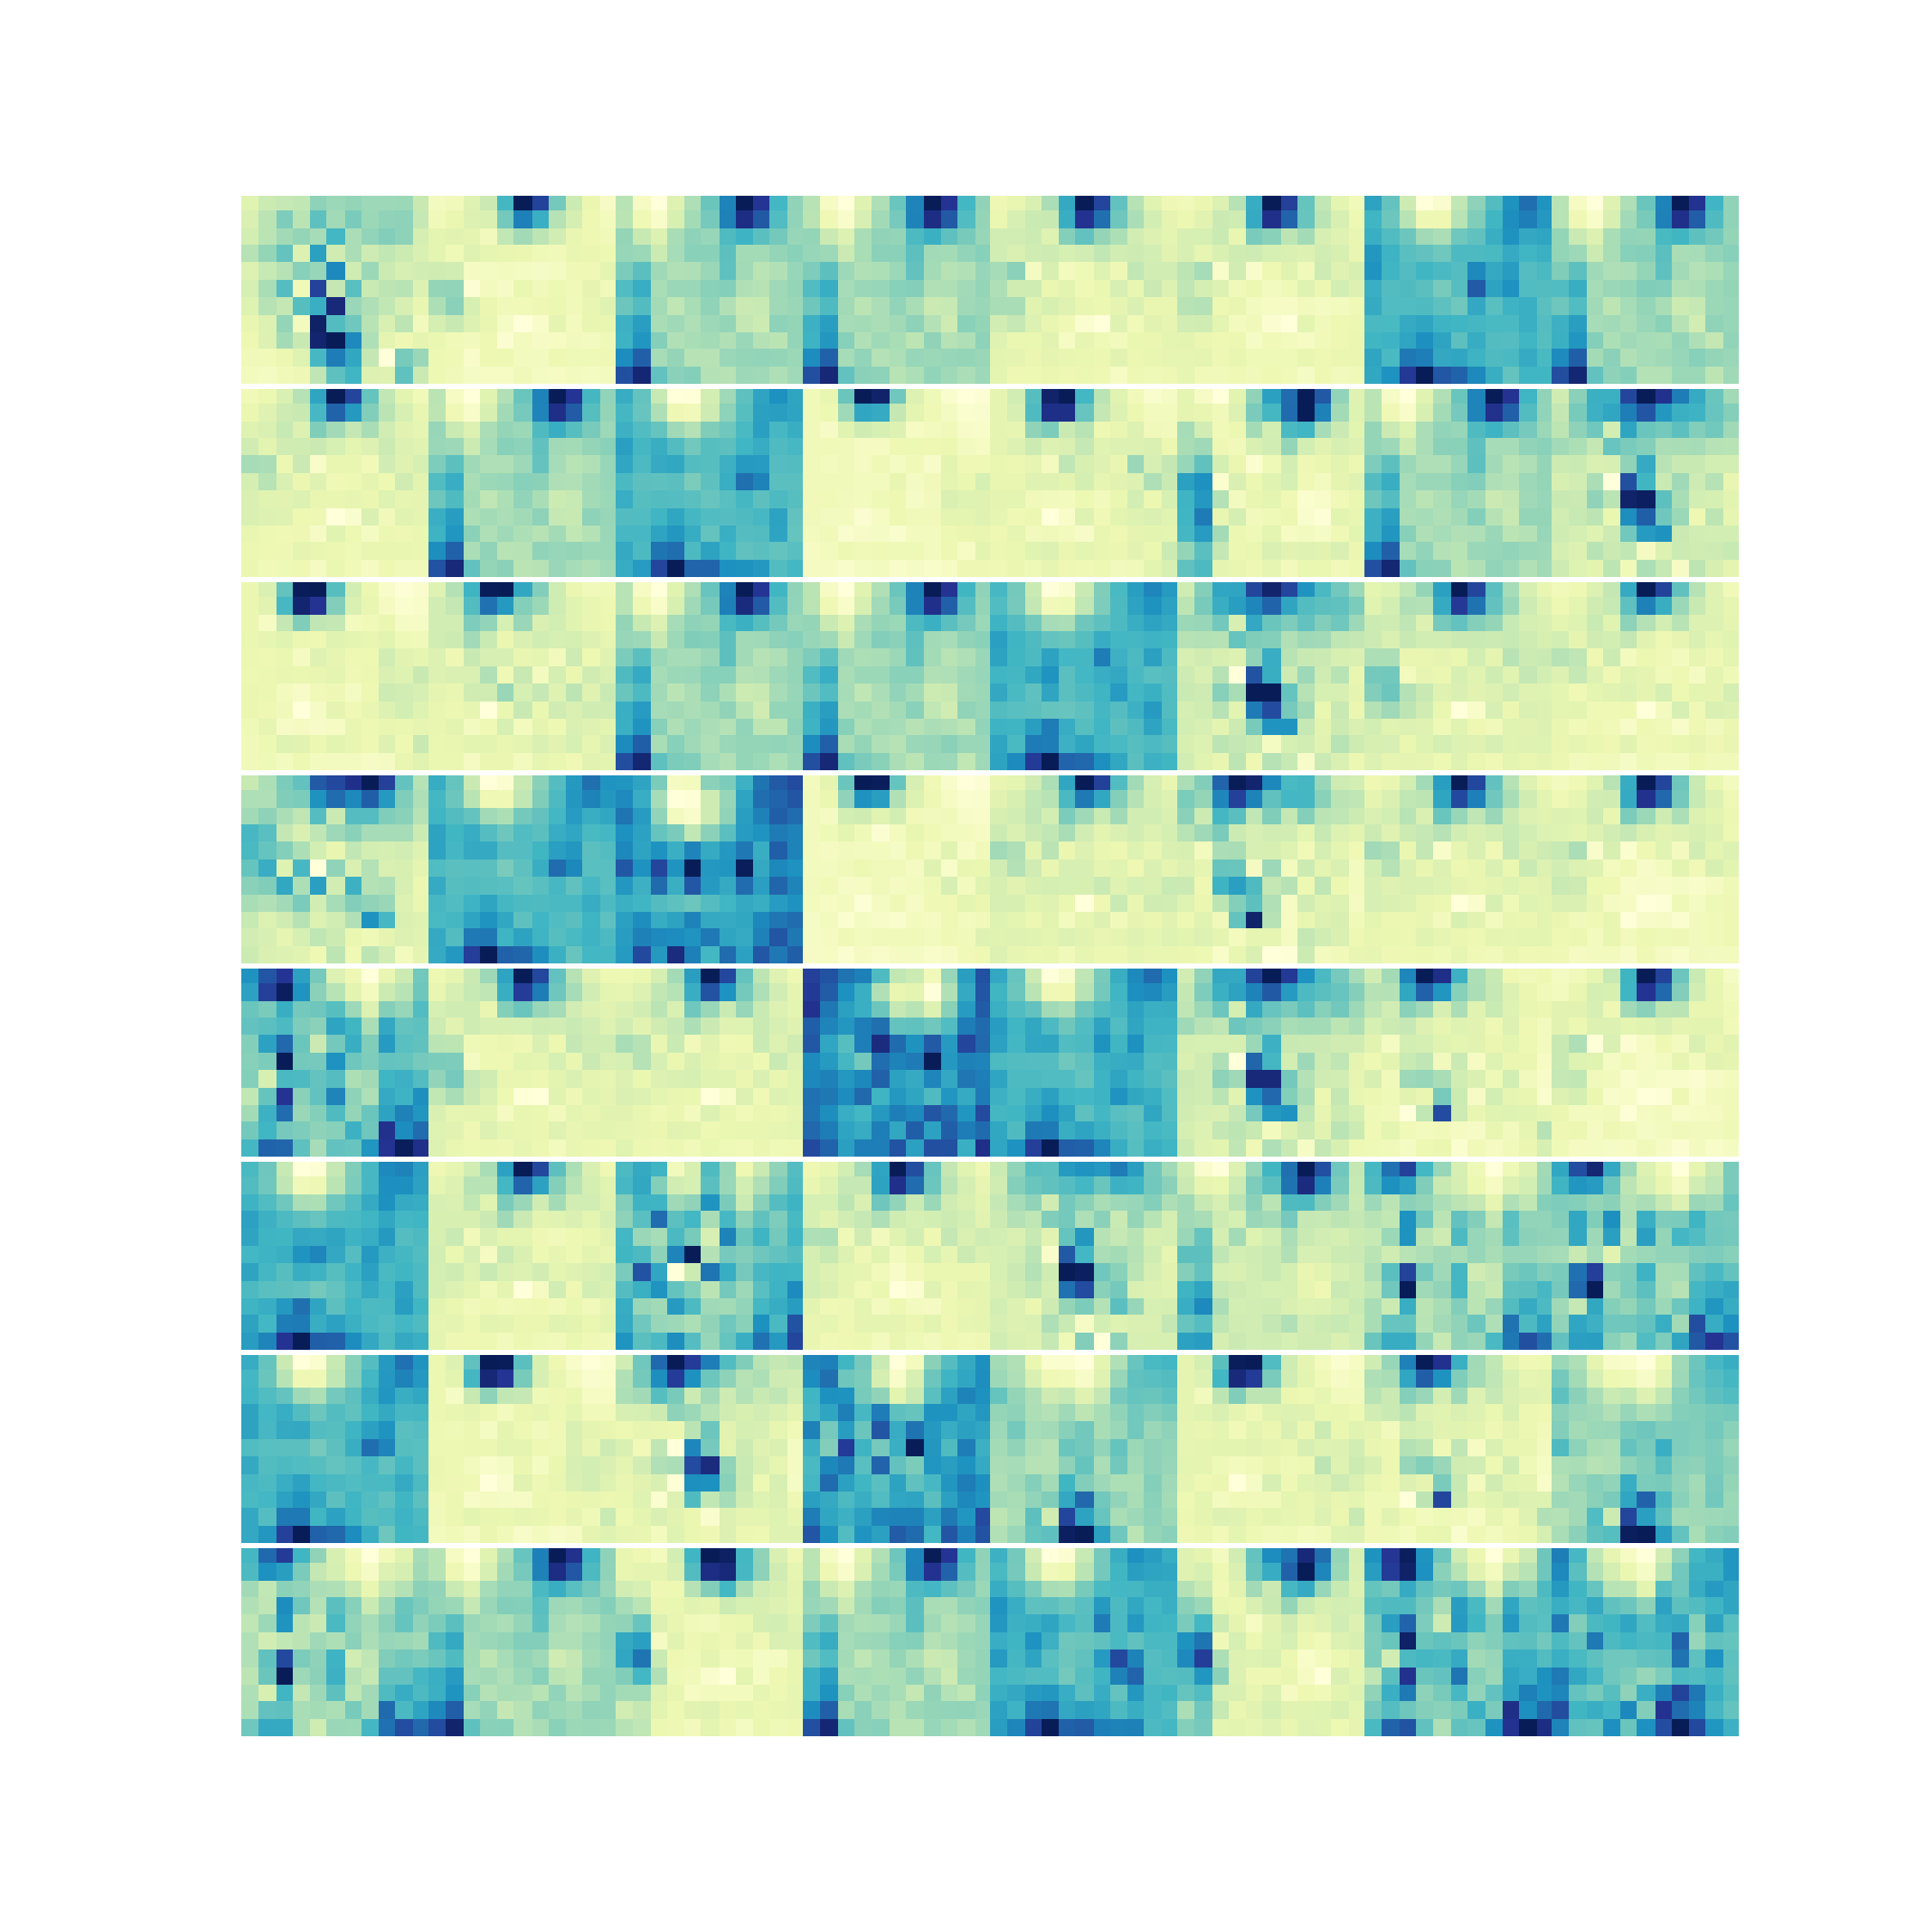
\includegraphics[width=0.5\textwidth]{figures/conv-filts.pdf}
      }
      \subfloat[Convolved Jet Image differences\label{subfig:convolvedfilters}]{
        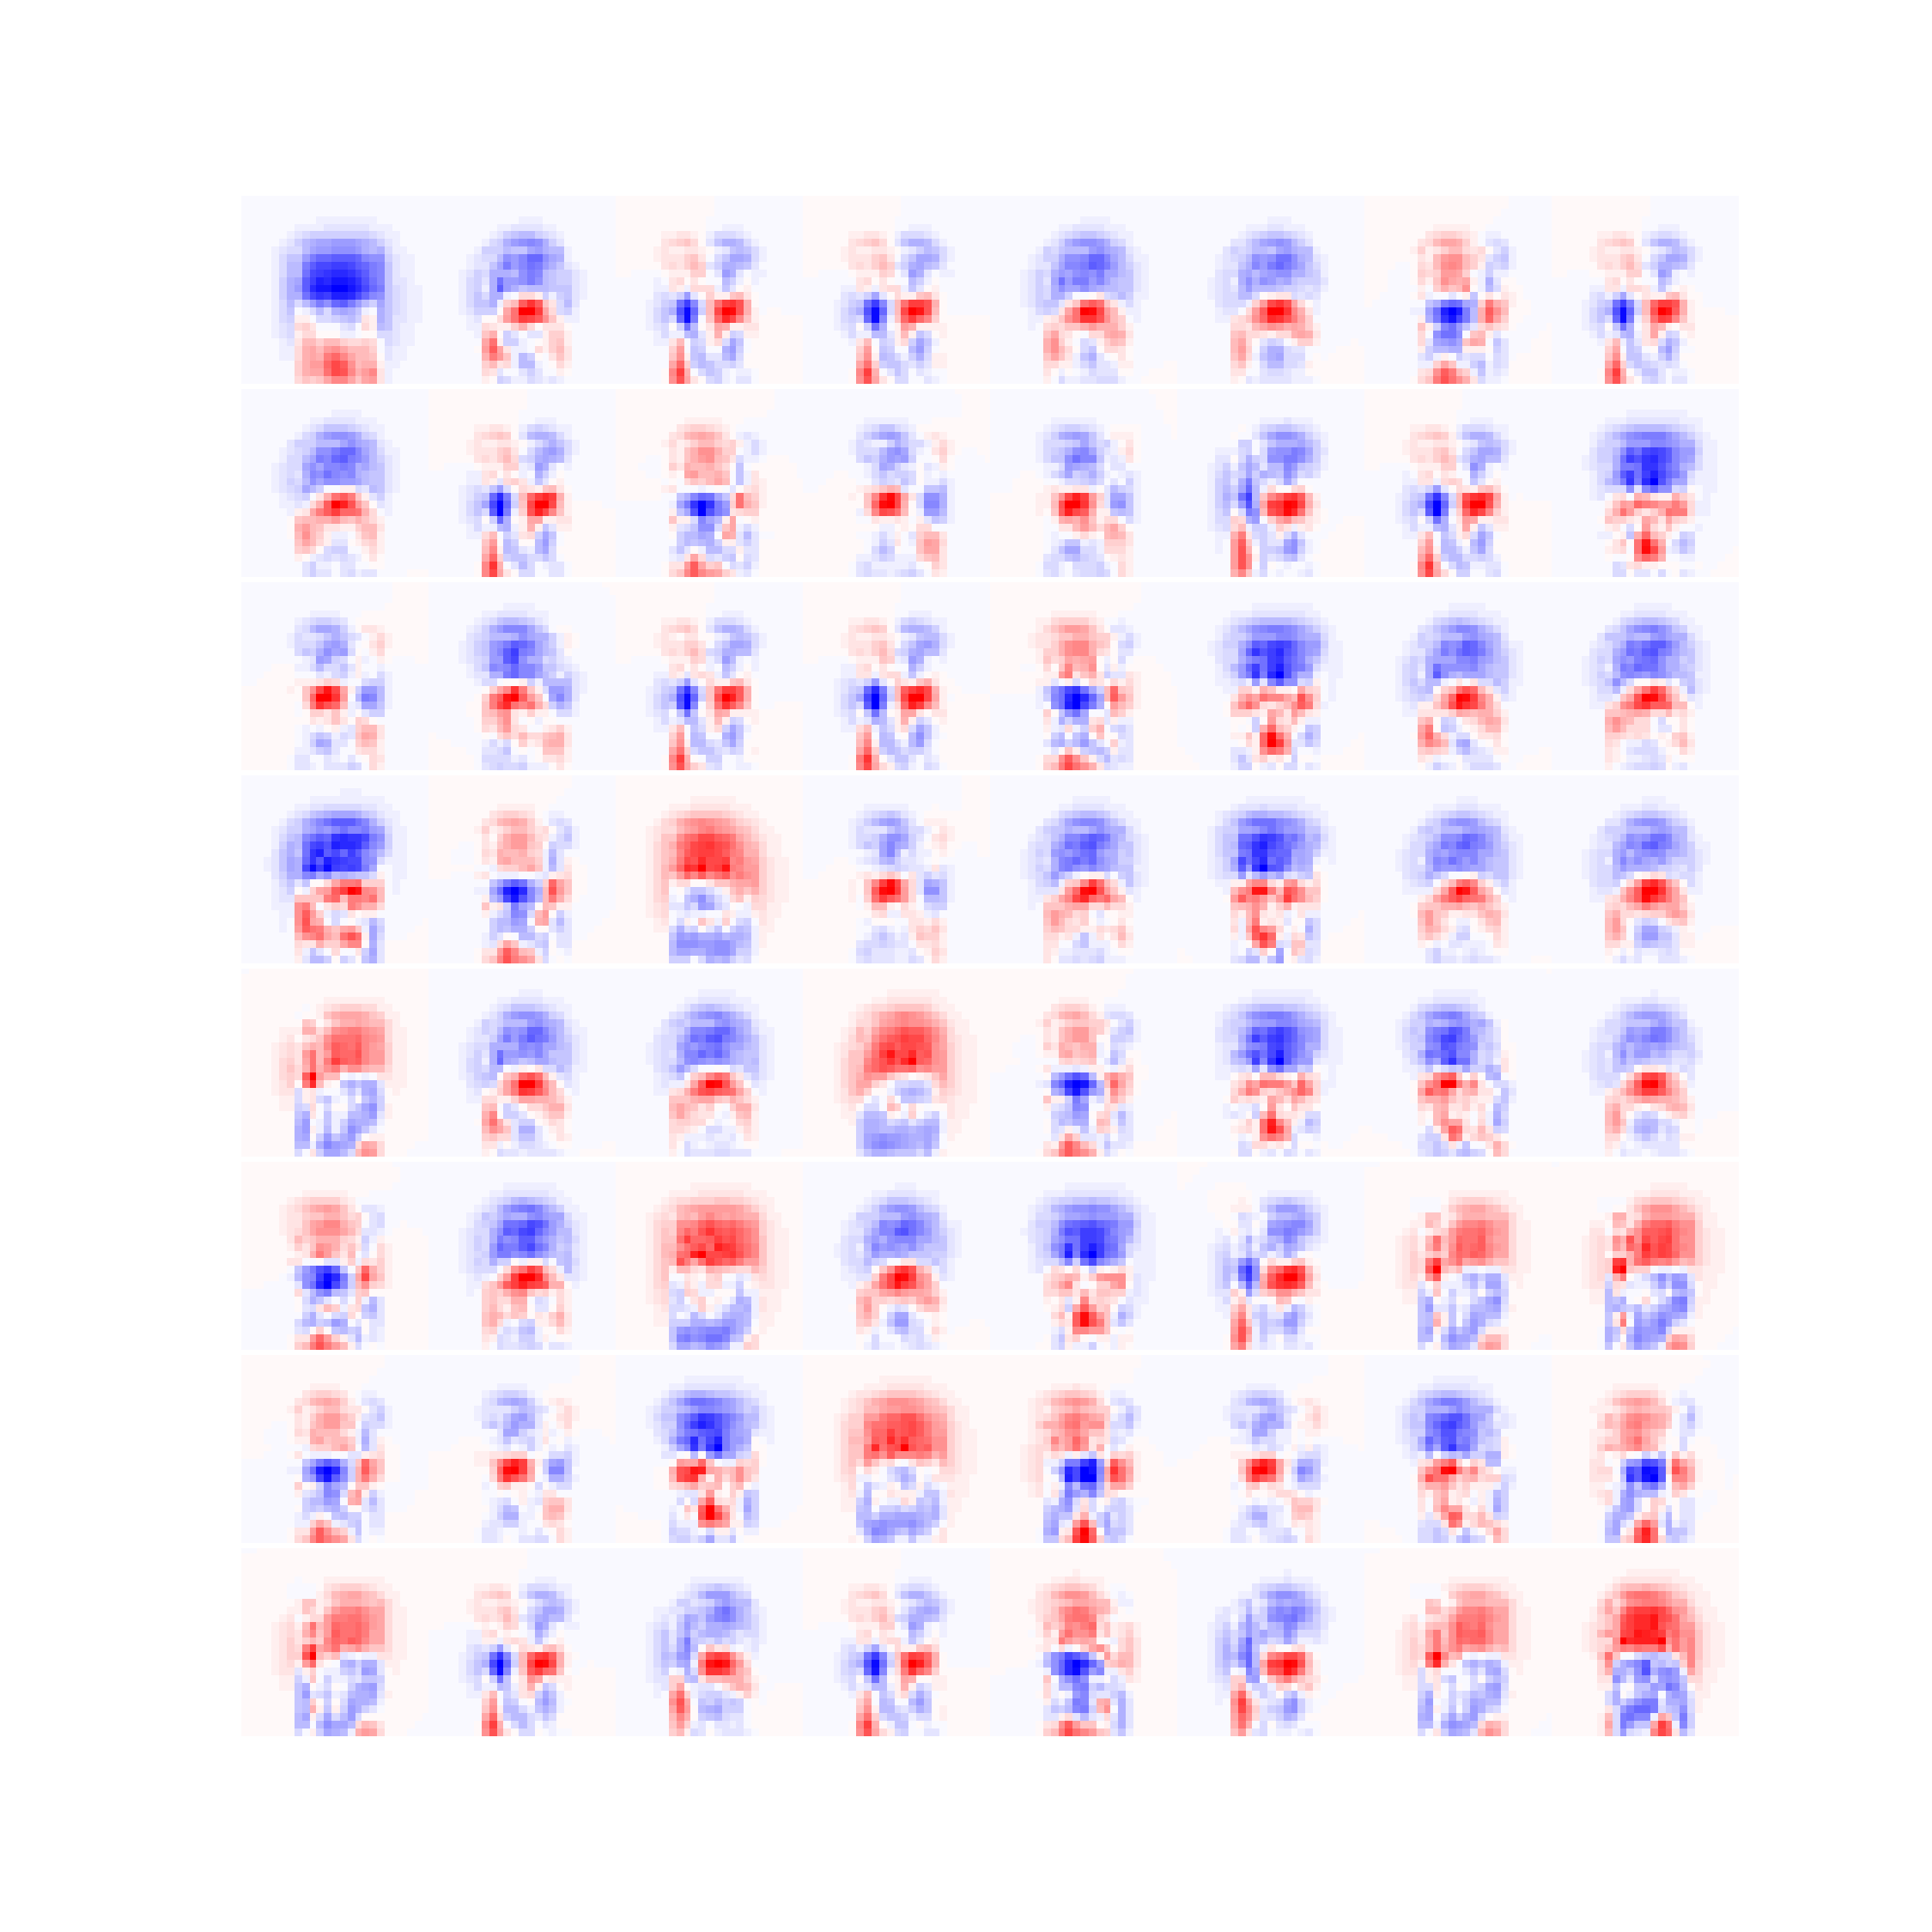
\includegraphics[width=0.5\textwidth]{figures/conv-diffs-global.pdf}
      }
      \caption{Convolutional Kernels (left), and convolved feature differences in jet images (right)}
      \label{fig:convkernels}

    \end{center}
\end{figure}



Blah... linear correlations with pixels





\subsubsection{Physics in Deep Representations} % (fold)
\label{ssub:physics_in_deep_representations}


\begin{figure}[!htbp]
  \centering
  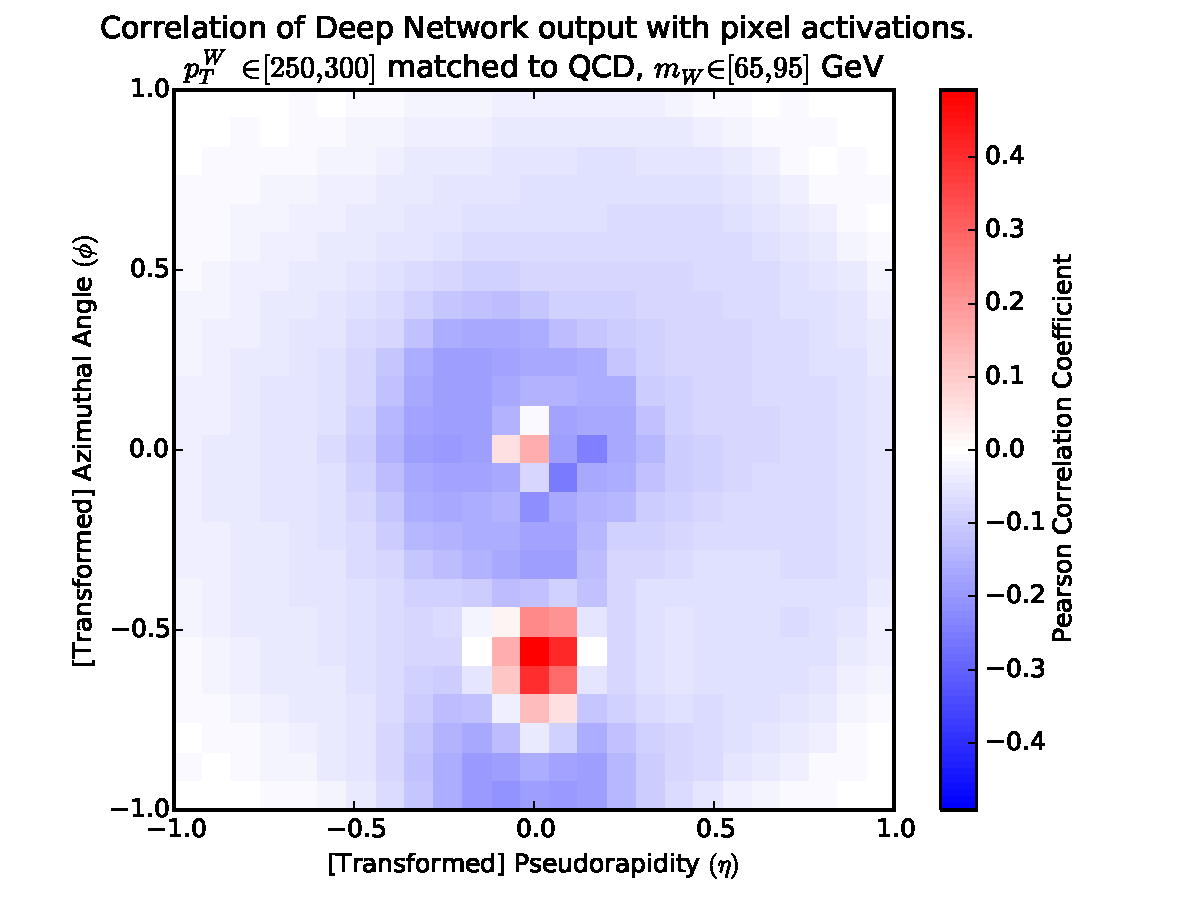
\includegraphics[width=0.95\textwidth]{figures/pixel-activations-corr.pdf}
  \caption{Per-pixel linear correlation with DNN output}
  \label{fig:corr}
\end{figure}


\begin{figure}[bt]
  \begin{center}
      \subfloat[Sculpted QCD $\Delta R$ distribution\label{fig:sculpteddR}]
      {
        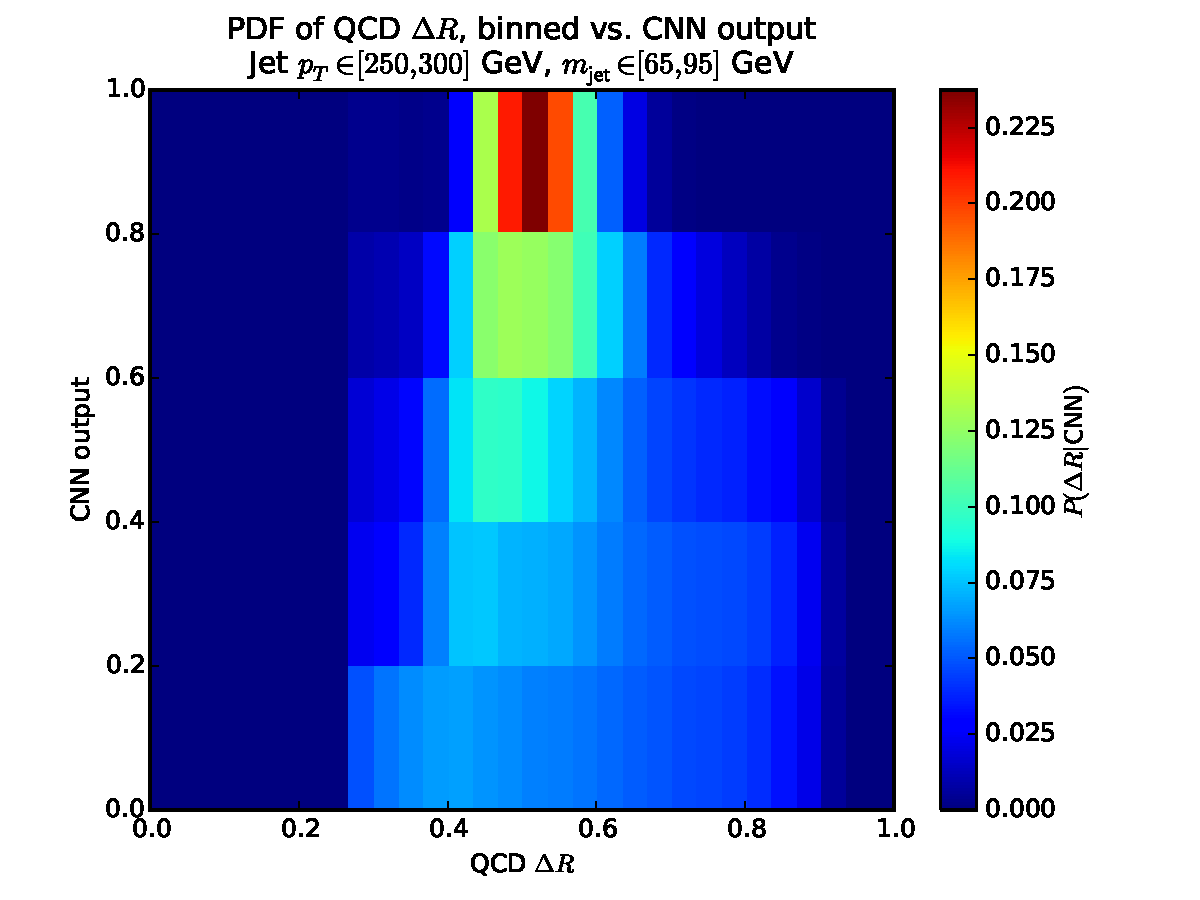
\includegraphics[width=0.5\textwidth]{figures/dR-dist-by-CNN.pdf}
      }
      \subfloat[Sculpted QCD $\tau_{21}$ distribution\label{fig:sculptednsj}]
      {
        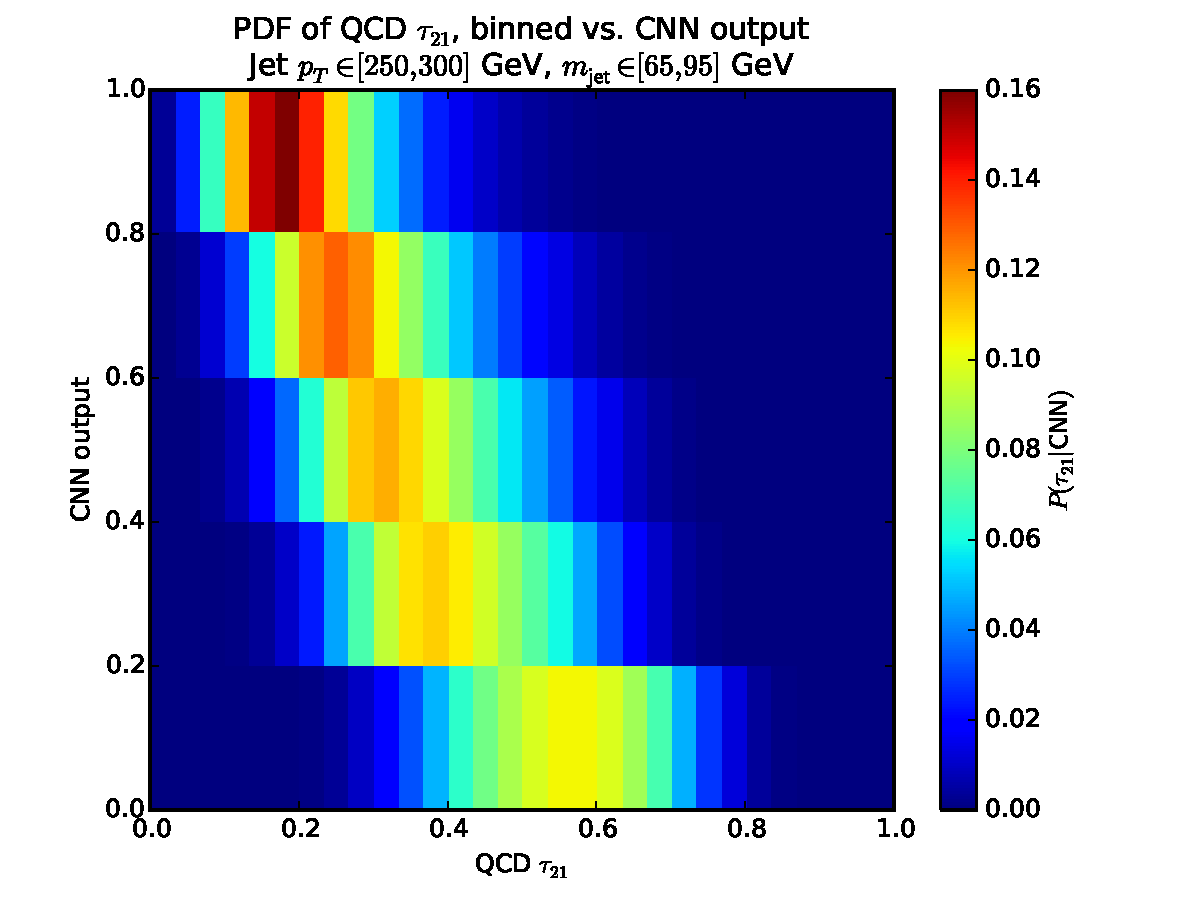
\includegraphics[width=0.5\textwidth]{figures/tau-dist-by-CNN.pdf}
      }
      \\
      \subfloat[Sculpted QCD mass distribution\label{fig:sculptedmass}]
      {
        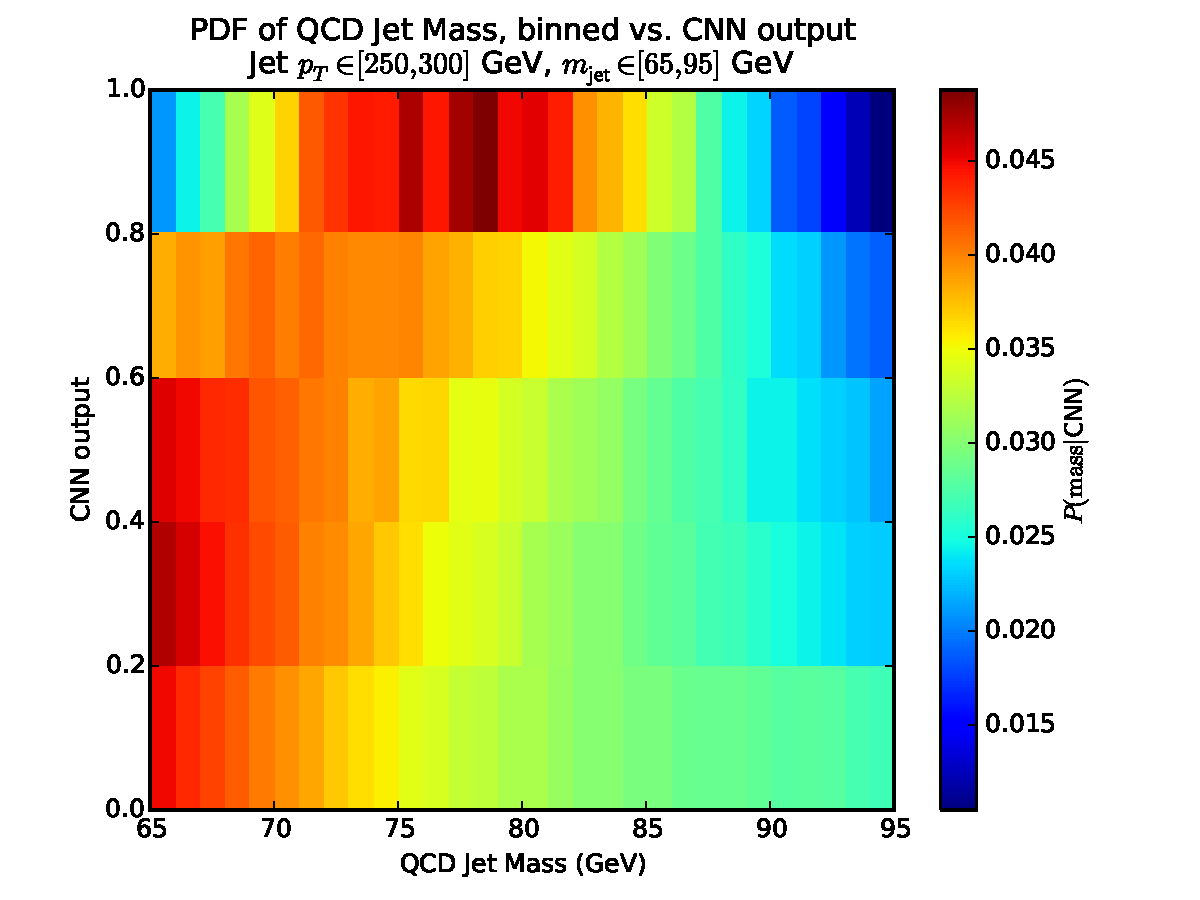
\includegraphics[width=0.5\textwidth]{figures/mass-dist-by-CNN.pdf}
      }

      \caption{Sculpted QCD distributions}
      \label{fig:qcdsculpt}

    \end{center}
\end{figure}





% subsubsection physics_in_deep_representations (end)

% subsection coarse_studies (end)

\subsection{Flat Hypercube Studies} % (fold)
\label{sub:flat_hypercube_studies}


Here, we see the ROC blah...

\begin{figure}[htbp]
  \centering
  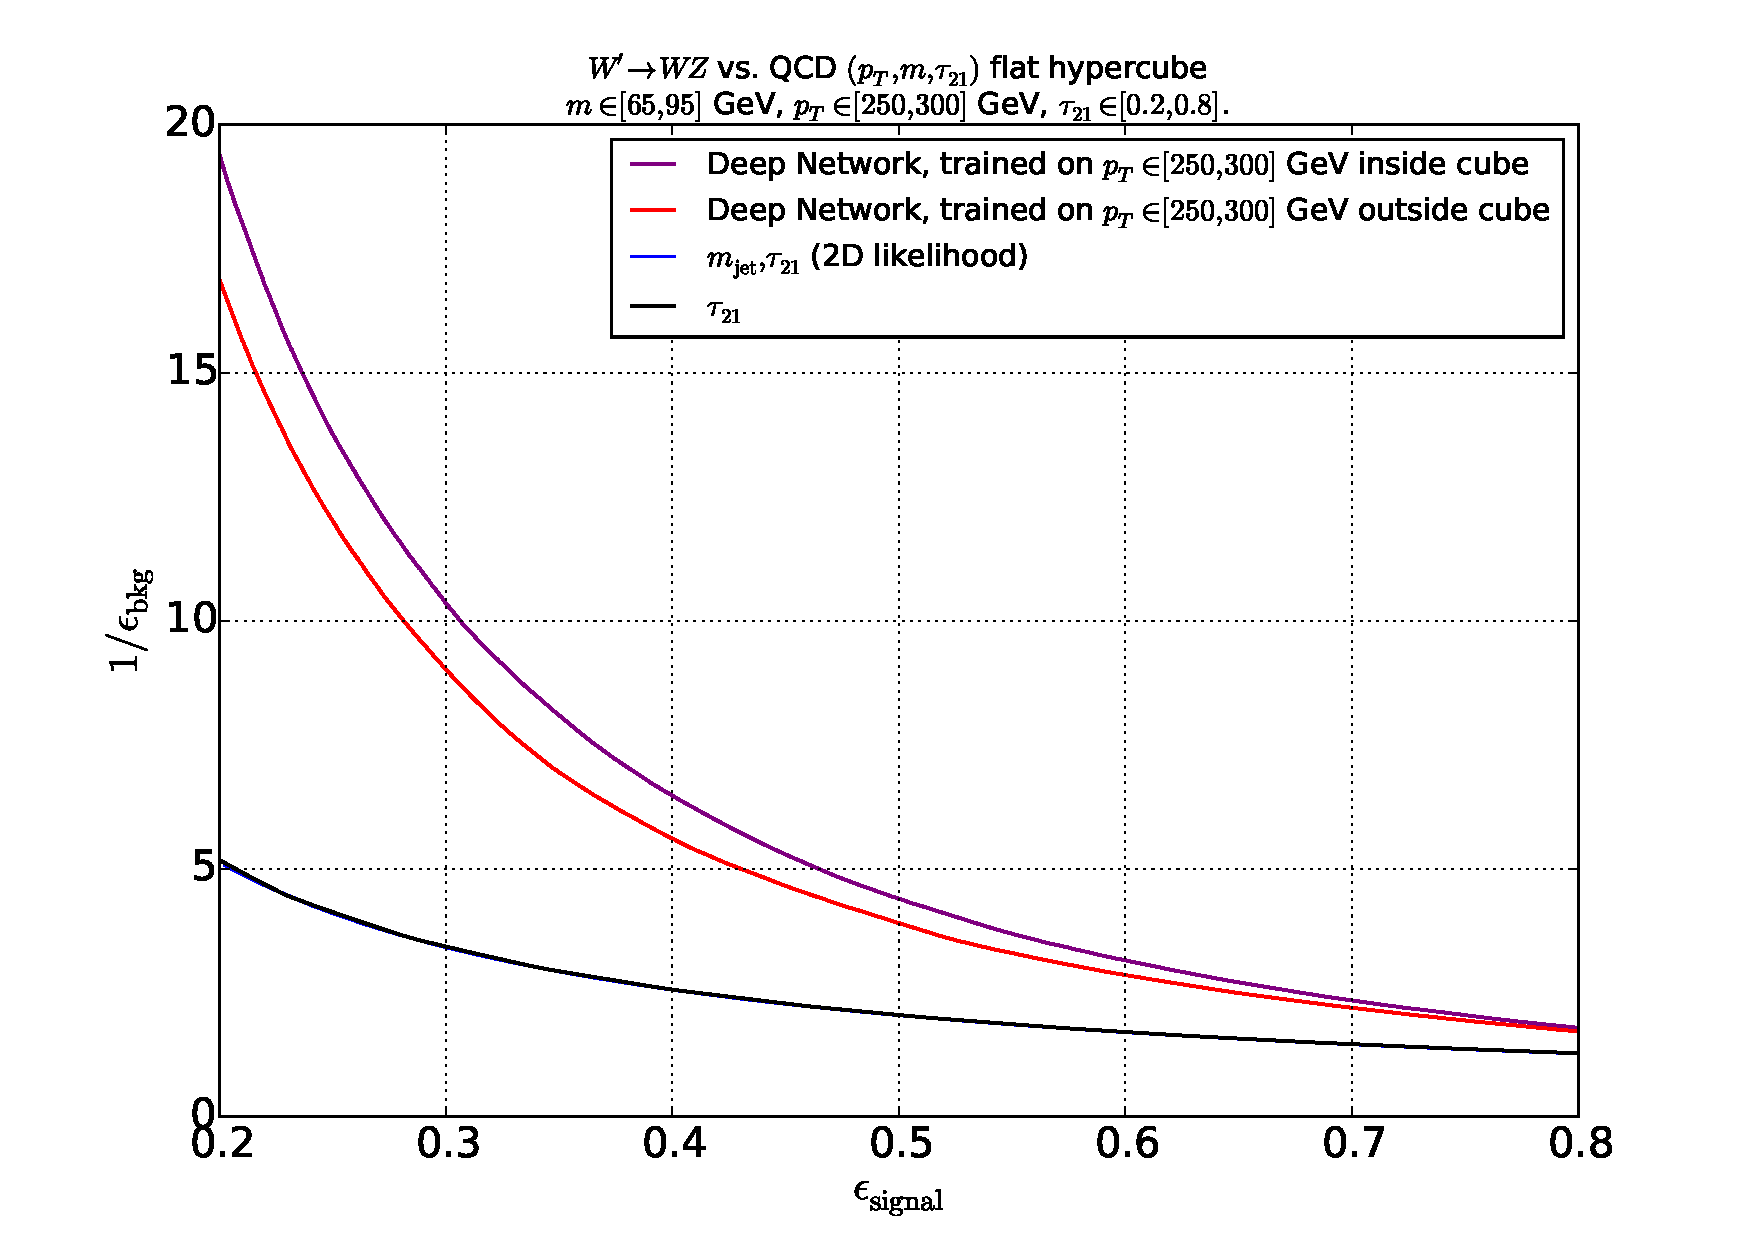
\includegraphics[width=0.95\textwidth]{figures/roc-cube-inside.pdf}
  \caption{ROC Curve for weigth-flattened hypercube, with $m\in[65, 95]\mathsf{GeV}$,  $p_T\in[250, 300]\mathsf{GeV}$, and  $\tau_{21}\in[0.2, 0.8]$}
  \label{fig:rocCube}
\end{figure}

% subsection flat_hypercube_studies (end)



\subsection{Small Window Studies} % (fold)
\label{sub:small_window_studies}


\begin{figure}[bt]
  \begin{center}
  
      \subfloat[Average $W'\rightarrow WZ$ image \label{subfig:sig_window}]{
        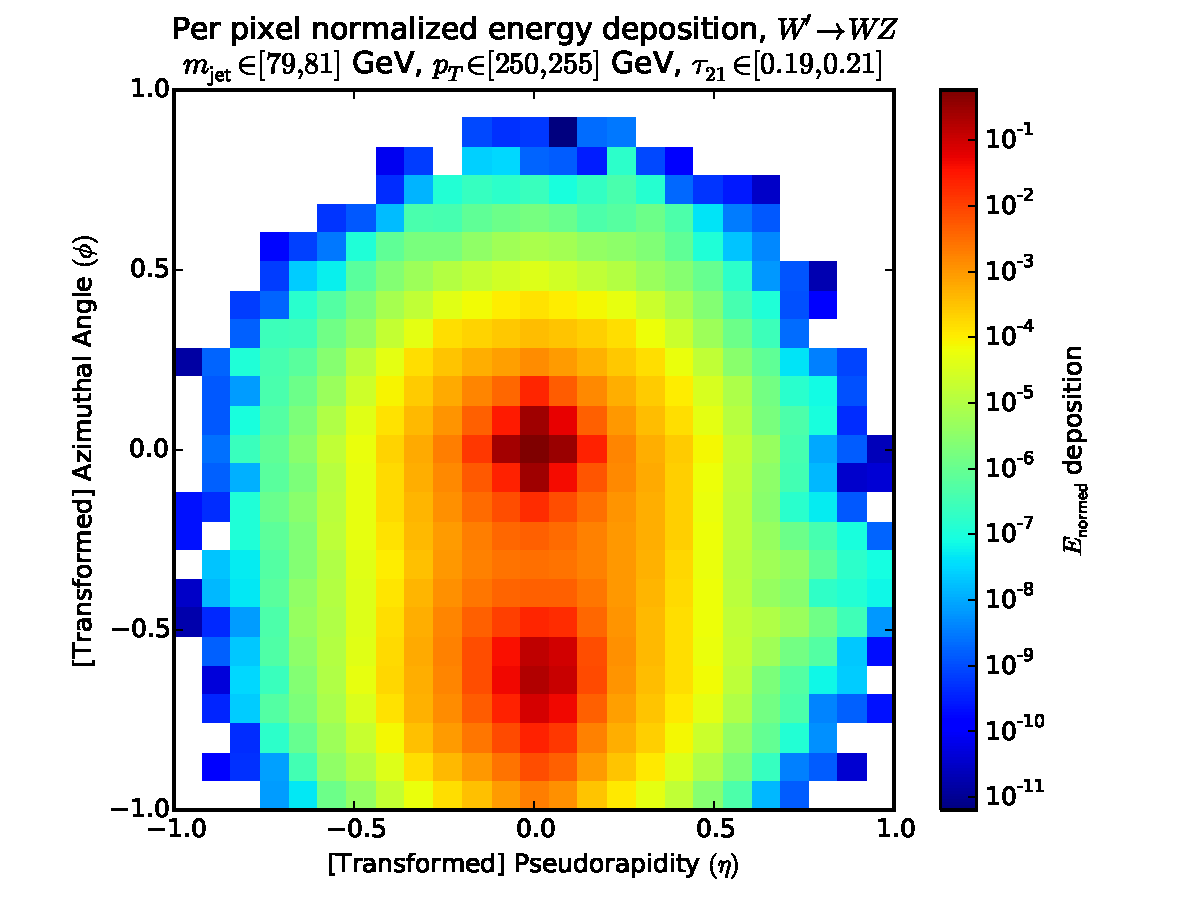
\includegraphics[width=0.5\textwidth]{figures/avg-benwindow-sig.pdf}
      }
      \subfloat[Average QCD image \label{subfig:bkg_window}]{
        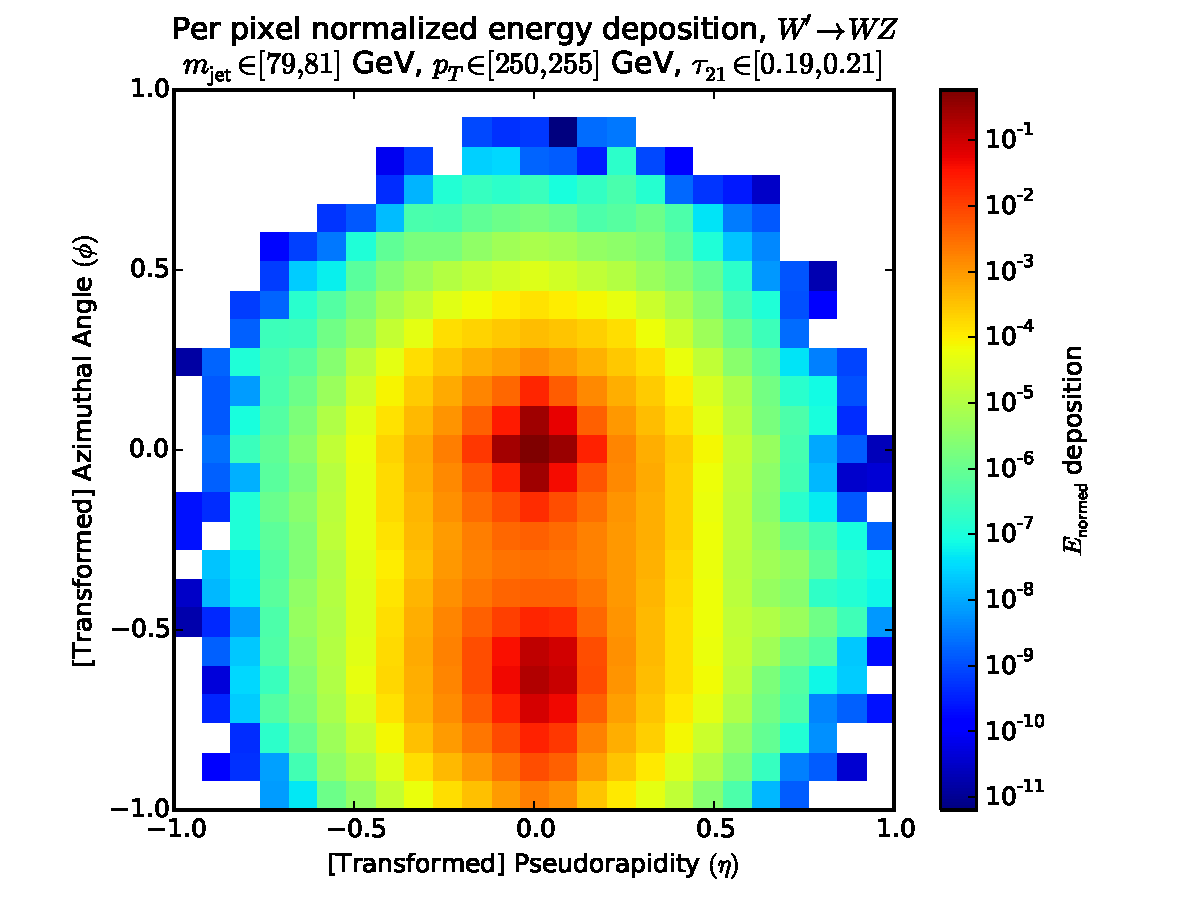
\includegraphics[width=0.5\textwidth]{figures/avg-benwindow-sig.pdf}
      } \\
      \subfloat[Average image difference \label{subfig:windowdiff}]{
        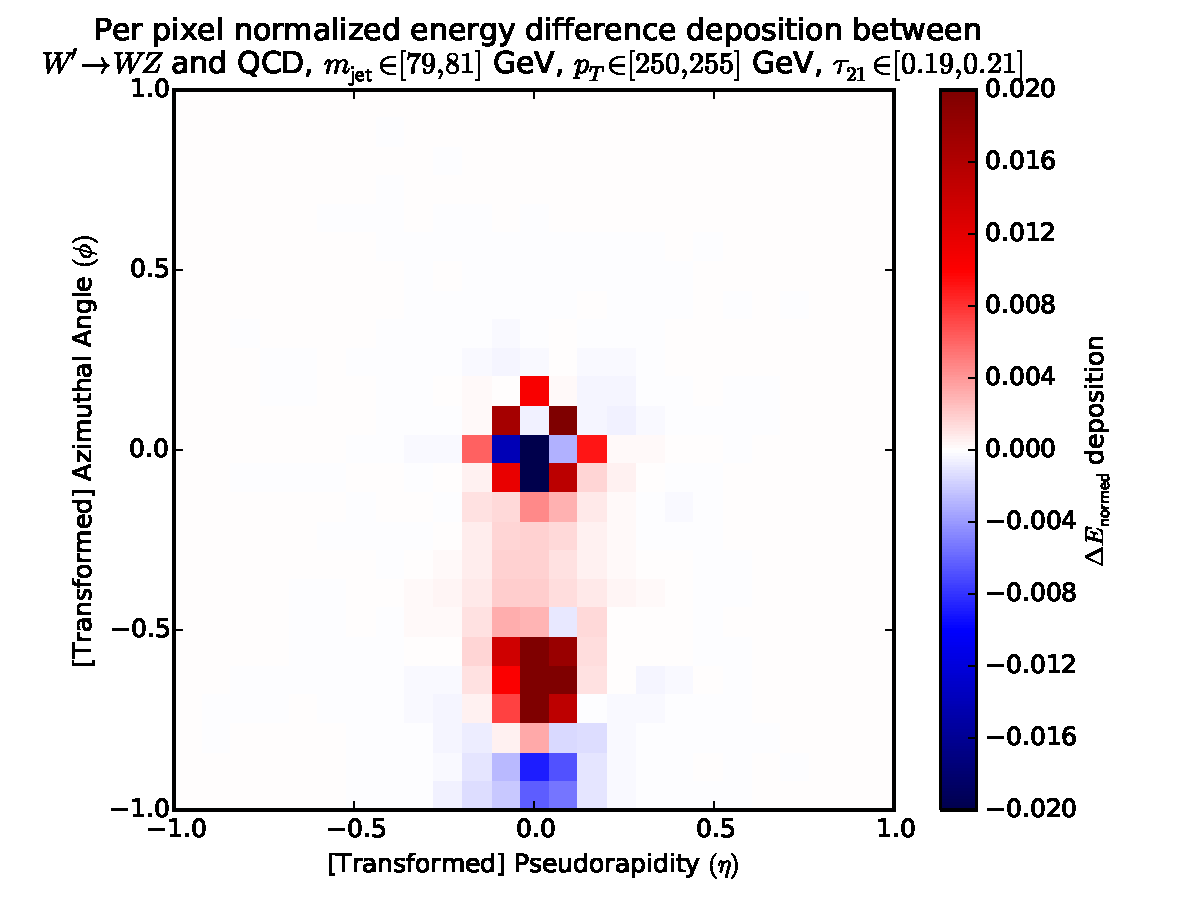
\includegraphics[width=0.5\textwidth]{figures/avg-benwindow-diff-clipped.pdf}
      }
      \caption{$W'\rightarrow WZ$ (left) and QCD (right) average jet-images, and Signal - Background image difference (bottom)
      \label{fig:meanImagesWindow} }
    \end{center}
\end{figure}  


Performance inside the window, use a Fisher Discriminant...

\begin{figure}[htbp]
  \centering
  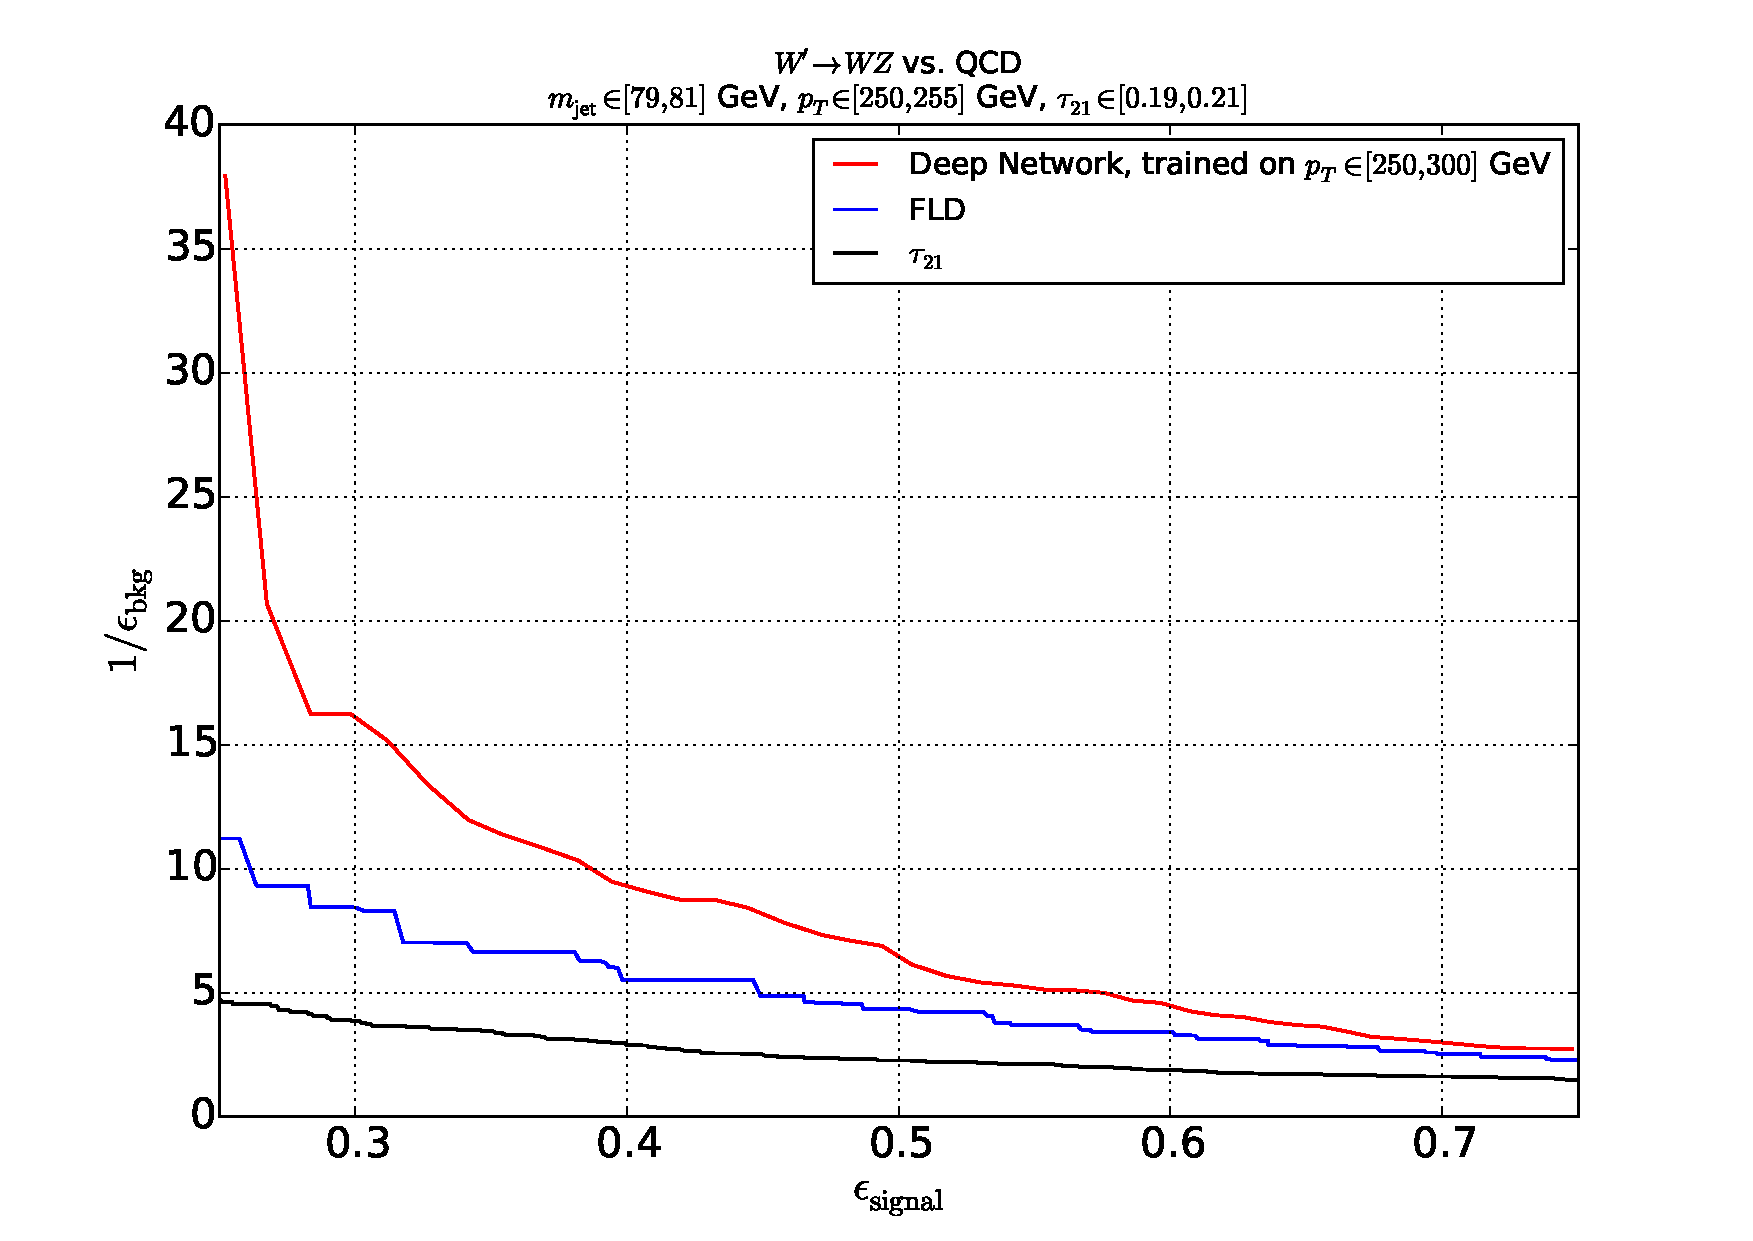
\includegraphics[width=0.95\textwidth]{figures/augwindow-roc.pdf}
  \caption{Receiver Operating Characteristic (ROC) over window sample}
  \label{fig:rocWindow}
\end{figure}

\subsubsection{Understanding what we learn} % (fold)
\label{ssub:understanding_what_we_learn}

\begin{figure}[htbp]
  \centering
  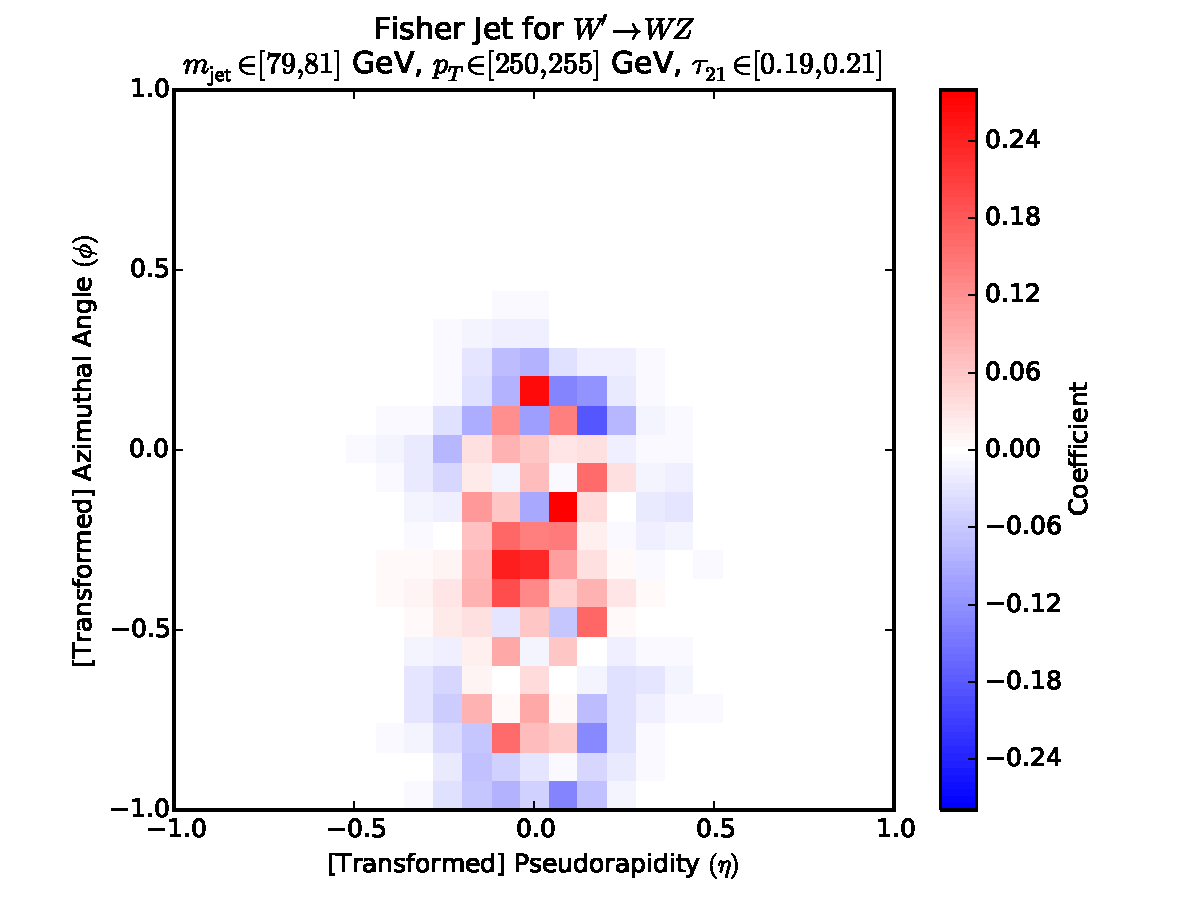
\includegraphics[width=0.65\textwidth]{figures/fld-benwindow.pdf}
  \caption{caption}
  \label{fig:fldWindow}
\end{figure}

\begin{figure}[htbp]
  \centering
  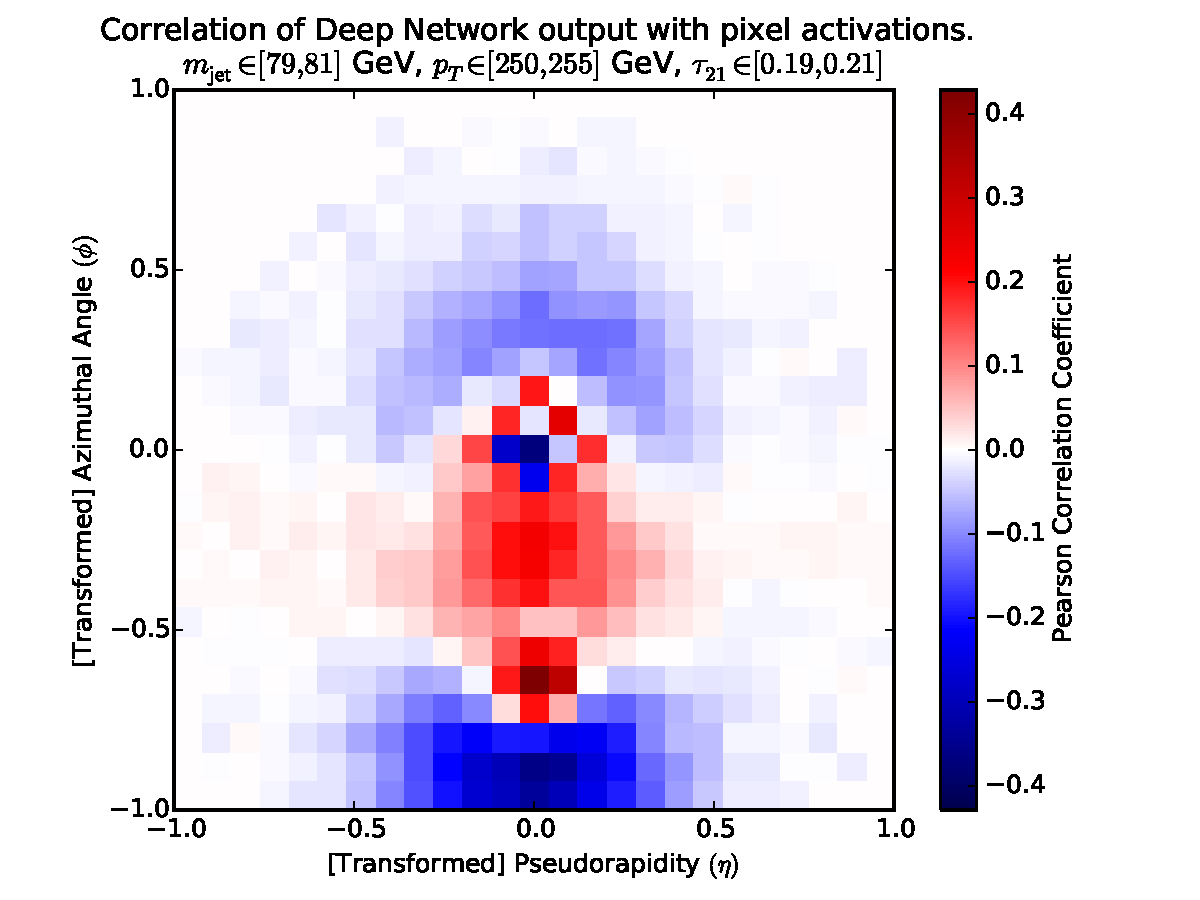
\includegraphics[width=0.65\textwidth]{figures/pixel-activations-corr-benwindow.pdf}
  \caption{caption}
  \label{fig:corrWindow}
\end{figure}


\begin{figure}[htbp]
  \centering
  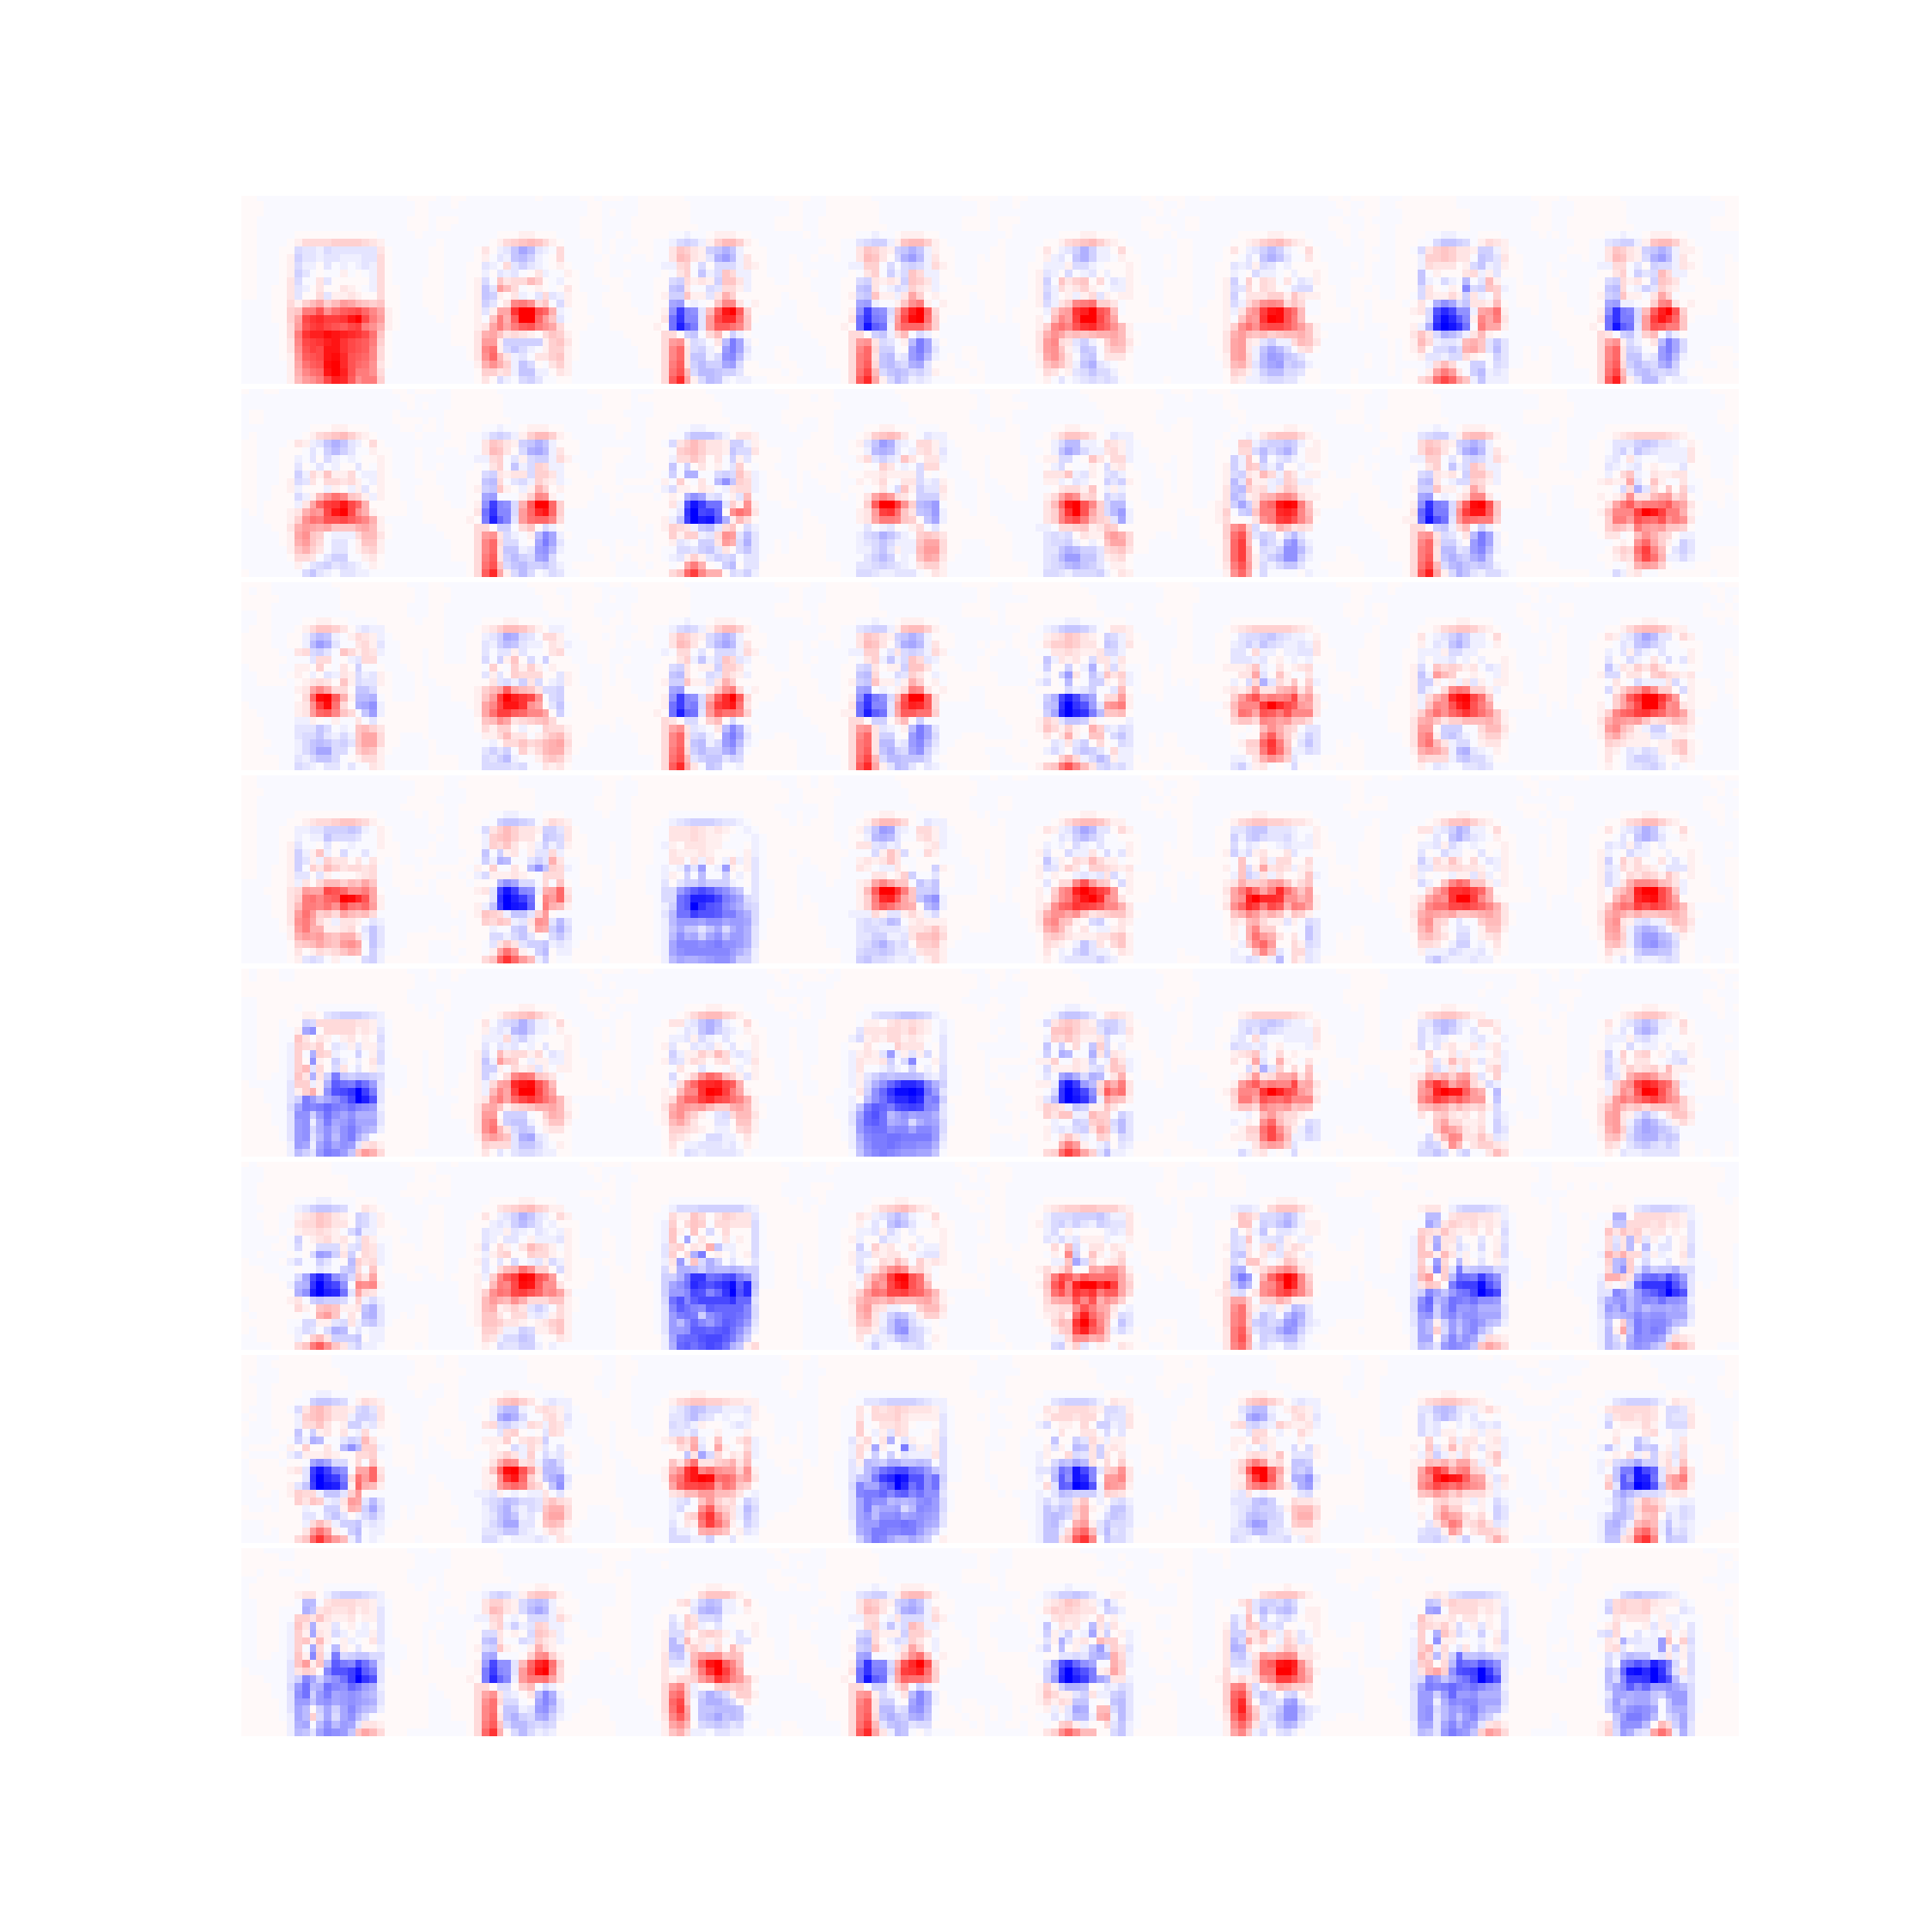
\includegraphics[width=0.95\textwidth]{figures/conv-diffs-ben-window.pdf}
  \caption{caption}
  \label{fig:convkernelsWindow}
\end{figure}
% subsubsection understanding_what_we_learn (end)

% subsection small_window_studies (end)





% section studies (end)
